\documentclass[compress,10]{beamer}
\mode<presentation>
\usepackage{multicol}
\usepackage{multirow}
\usepackage{bm}
\usepackage{amssymb}
\usepackage{amsmath}
\usepackage{hyperref}
\hypersetup{colorlinks=false}
\usepackage{rotating} %allow for rotation of plots
\usepackage{fancybox}
\usepackage{pgf,pgfarrows,pgfnodes}
\usepackage{caption}
%%\usepackage{subcaption}

\usepackage{pgf,pgfarrows,pgfnodes}
\usepackage{beamerthemesplit} 
\usetheme{Berlin}
\usecolortheme{default}
%%  mds commented out the line below as it led to error messages:
%% LaTeX Error: Too many math alphabets used in version normal.
%% see  http://tex.stackexchange.com/questions/3676/too-many-math-alphabets-error
%%  mds dangerous\usepackage{MnSymbol,wasysym}
%\usecolortheme{LHCbPresentation}

\setbeamertemplate{navigation symbols}{}%Turn off Navigation Symbols
\selectcolormodel{rgb}
\definecolor{LHCb dark}{rgb}{0.0000,0.3412,0.6549}%From LHCb logo
\definecolor{UC red}{rgb}{0.8196,0.1176,0.2314} % from logo
\definecolor{brickred}{rgb}{0.8, 0.25, 0.33}

\def\baselinestretch{0.90}


%\def\insertnavigation#1{\relax}
%===========================================
%Put Frame Numbers in Bottom Right Corner
\newcommand*\oldmacro{}%
\let\oldmacro\insertshorttitle%
\renewcommand*\insertshorttitle{%
  \oldmacro\hfill%
  \insertframenumber\,/\,\inserttotalframenumber}
%============================================
%allow manual positioning of images
\newcommand{\putat}[3]{\begin{picture}(0,0)(0,0)\put(#1,#2){#3}\end{picture}}
%============================================
\title{S2I2 and US ATLAS Software \& Computing Support }
\author[Peter Elmer, Mark Neubauer, and Mike Sokoloff]
{
 \textcolor{LHCb dark}{\bf  Peter Elmer, Mark Neubauer, and Mike Sokoloff}
}
%% mds \institute[\textcolor{white}{The University of Cincinnati}]
%% mds {\textcolor{black}
%% mds {The  University of Cincinnati}
%% mds }
%
\date{August, 2016}

\begin{document}

%========================================================================
%Make Title Page
\begin{frame}[noframenumbering]
	\titlepage
\end{frame}
%=====================================================================
%%%%%%%%%%%%%%%%%
\begin{frame}[fragile]{Software and Computing for the HL-LHC Era}{}
{\footnotesize
The DOE and NSF jointly invest $ \approx \$ 35 $M/year in
ATLAS and CMS software and computing, about half in hardware plus operations,
about half in software professionals.
The LHC funding agencies, worldwide, invest about $ \$ 150 $M/year
in these enterprises.
In 2014, the LHC experiments used almost 175 PB of tape storage and
slightly more disk storage.
The event rate anticipated for the HL-LHC era is 100 times greater,
and even assuming the experiments significantly reduce the
amount of data stored per event,
the total size of the datasets will be well into the exabyte
scale;
they will be constrained primarily by costs and funding levels,
not by scientific interest.
One long-term goal of a HEP $ S^2 I^2 $
will be
maximizing the return-on-investment to enable break-through
scientific discoveries using the  HL-LHC detectors.
}  %%  end \footnotesize
\end{frame}
%=====================================================================
%%%%%%%%%%%%%%%%%
\begin{frame}[fragile]{NSF Scientific Software Innovation Institute (S2I2)}{}

A possible path to a software upgrade project for HL-LHC with NSF}

{\footnotesize
\textcolor{brickred}{\bf The primary goal of the $ S^2 I^2 $ conceptualization 
process is to understand
the software requirements and challenges related to
the high-luminosity LHC and to prepare a strategic plan for addressing them.}
}  %%  end \footnotesize
\end{frame}
%=====================================================================
%%%%%%%%%%%%%%%%%
\begin{frame}[fragile]{A Community White Paper }{}
{\footnotesize
The {\bf Community White Paper (CWP)} will describe a global
vision for software and computing for the HL-LHC era.
It will discuss issues  common to
the LHC community  and  those that  are specific
to the individual experiments.
Many of the topics discussed here will address issues
required for a HEP $ S^2 I^2 $ implementation
proposal.
These will include
\begin{itemize}
  \item
    a broad overview of the grand challenge science of the HL-LHC;
  \item
    how new approaches to computing and software can enable and
    radically extend the physics reach of the detectors;
  \item
    \textcolor{brickred}{\bf
    what computing and software research will be required} so that
    computing and software Technical Design Reports
    can be prepared several years before Run 4 of the LHC begins;
    this will include studies of hardware and software architectures
    and life-cycle processes and costs.
   \item
    \textcolor{brickred}{\bf
    identify specific software elements and frameworks} that will
    be required for the HL-LHC era which can be built and tested
    during Run 3.
   \item
     \textcolor{brickred}{\bf
     organizational issues for the common software and for
     coordinating research of common interest}, even when the
     final products will be specific to individual experiments.
\end{itemize}
}  %% end of \footnotesize

\end{frame}

%=====================================================================
%%%%%%%%%%%%%%%%%
\begin{frame}[fragile]{NSF $S^2 I^2 $ Strategic Plan - I }{}
{\footnotesize
The separate {\bf Strategic Plan} will identify areas where the 
U.S.\ university
community can provide leadership and will discuss
those issues required for an $ S^2 I^2 $
which are not (necessarily) relevant to the larger community.
Topics will include:
 \begin{itemize}
   \item
     \textcolor{brickred}{\bf
     where does the U.S.\ university community already have
     expertise and important leadership roles;}
   \item
     which software elements and frameworks would provide
     the best educational and training opportunities
     for students and postdoctoral fellows;
   \item
     what  types of programs (short courses, short-term
     fellowships, long-term fellowships, etc.)
     might enhance the educational
     reach of an $ S^2 I^2 $;
   \item
     \textcolor{brickred}{\bf
     possible organizational, personnel and management
     structures and operational processes};
    \item
     \textcolor{brickred}{\bf
     how the investment in an $ S^2 I^2 $ can be judged
     and how the investment can be sustained}
     to assure the scientific goals of the HL-LHC.
 \end{itemize}

}  %% end of \footnotesize

\end{frame}
%=====================================================================
%%%%%%%%%%%%%%%%%
\begin{frame}[fragile]{NSF $S^2 I^2 $ Strategic Plan - II }{}
{\footnotesize
Using the CWP as a stepping-off point, the Strategic Plan will also address
topics specific to proposed U.S. university efforts:
\begin{itemize}
 \item
  \textcolor{brickred}{\bf
  the scope of possible projects will be coordinated with
  other stake-holders, including DOE-funded laboratories}
  in the U.S.\ and international collaborators,
  to assure a coherent community-wide effort;
 \item
  the plan will identify possible management structures,
  mechanisms for continuing assessment,
  and appropriate education and outreach activities.
 \item
  \textcolor{brickred}{\bf
   development, testing and deployment
   methodologies, validation and verification processes,
   end usability and interface consideration,
   and required infrastructure and technologies};
 \item
   the requirements and necessary mechanisms for 
  \textcolor{brickred}{\bf human resource development},
   including integration
   of education and training, mentoring of students, postdoctoral fellows
   as well as
   software professionals, and proactively addressing diversity and
   broadening participation;
 \item
   \textcolor{brickred}{\bf
    potential risks} including risks associated with establishment and
   execution, necessary infrastructure
   and associated technologies, community engagement, and long-term
   sustainability.
\end{itemize}
}  %% end of \footnotesize

\end{frame}

%=====================================================================
%%%%%%%%%%%%%%%%%
\begin{frame}{A Nominal Timeline}{}
{\footnotesize
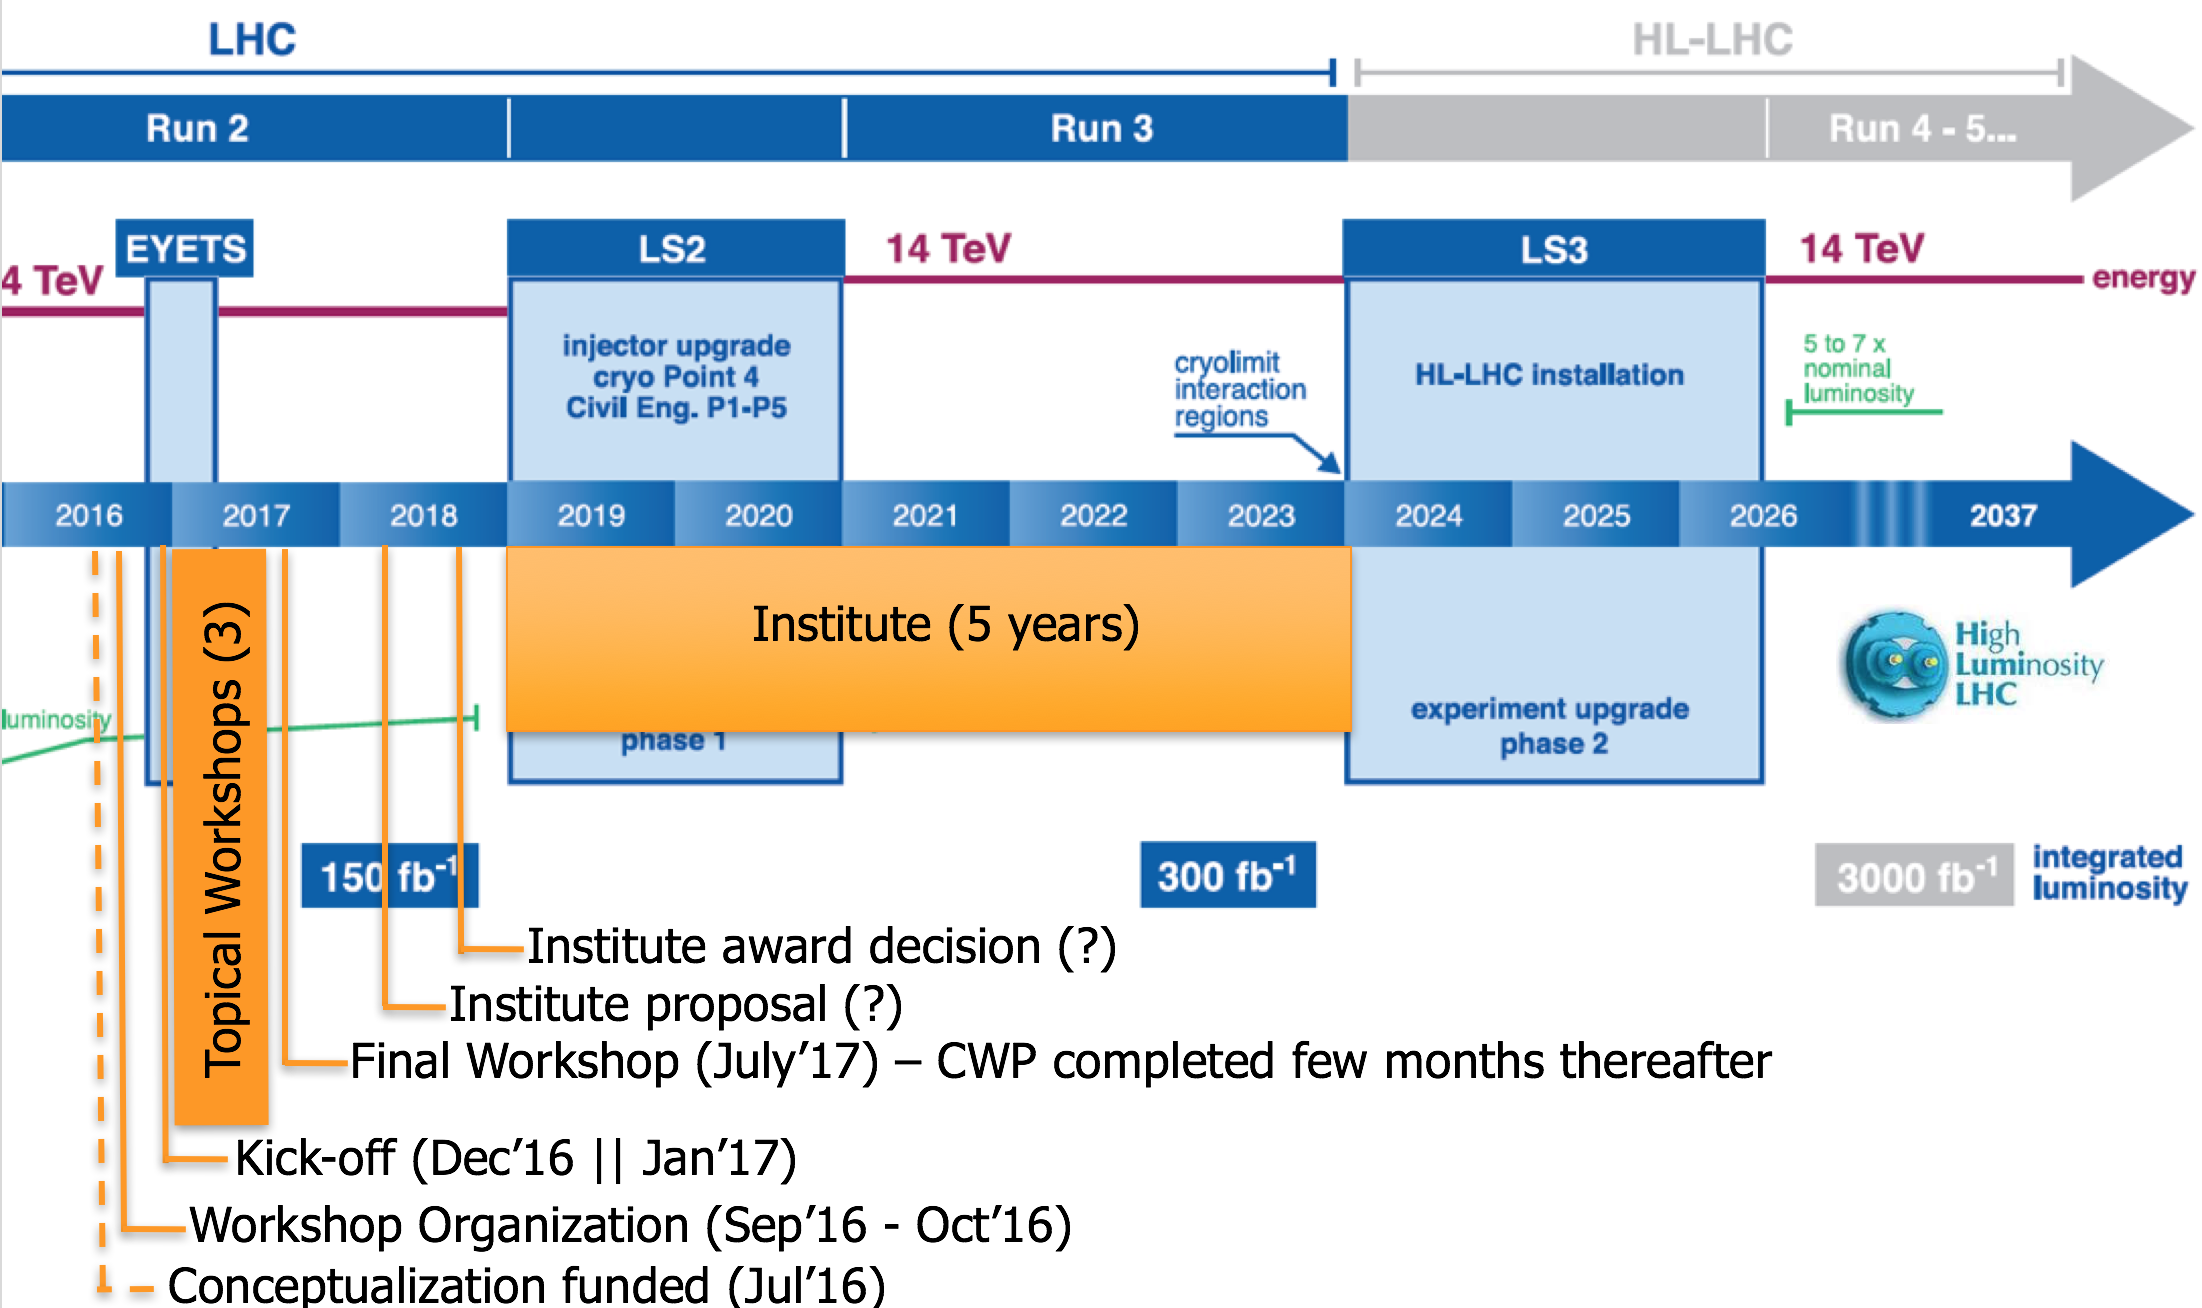
\includegraphics[width=1.0\textwidth]{S2I2_timeline.png}
}  %% end of \footnotesize

\end{frame}
%=====================================================================
%%%%%%%%%%%%%%%%%
\begin{frame}{Some Detector Simulation Issues}{}
{\footnotesize
The conceptualization proposal identifies \textcolor{brickred}{\bf
Detector Simulation} as a major focus area for discussion.
Challenges related to simulating high pile-up events include
\begin{itemize}
 \item
   \textcolor{brickred}{\bf CPU resources}
    for high statistics samples required to compare with
   real data for preparing triggers;
 \item
   \textcolor{brickred}{\bf high memory utilization};
 \item
   \textcolor{brickred}{\bf
   flexible simulation strategies} capable of providing a broad spectrum
   of precision of detector response, from ``fast" (parametric) simulation
   optimized for speed to full simulation in support of high precision
   measurements and new physics searches.
  \item
   software to \textcolor{brickred}{\bf emulate upgraded detectors}
   (including trigger systems) and
   suppport optimizing their configurations and calibration strategies.
  \item
   what \textcolor{brickred}{\bf mix of CPUs, GPUs, and/or FPGAs}
   will provide the 
   best bang-per-buck, including all life-cycle costs.
\end{itemize}
\vskip 0.1in
\noindent
\textcolor{brickred}{\bf Goals for today}:
Expand the list of topics for the simluations working groups to 
address and begin to think about how the work should be done.


}  %% end of \footnotesize

\end{frame}
%=====================================================================
%%%%%%%%%%%%%%%%%
%=====================================================================
%%%%%%%%%%%%%%%%%
\begin{frame}{Some Data Access and Management, Workflow,
and Resource Management Issues}{}
{\footnotesize
Data handling systems will need to scale to the multi-exabyte scale during
the HL-LHC era.
Issues to be addressed will include:
\begin{itemize}
 \item
  \textcolor{brickred}{\bf analyst access} to data and metadata;
 \item
  \textcolor{brickred}{\bf workflow management}
   systems capable of handling millions of jobs
  running on large numbers of heterogeneous, distributed computing resources;
 \item
  tools for measuring and monitoring \textcolor{brickred}{\bf networking 
  bandwidth and latency} between
  resource targets for use in job brokering;
 \item
  \textcolor{brickred}{\bf
  software-defined networking} technologies to enable efficient use of 
  resources;
 \item
  \textcolor{brickred}{\bf event-based data streaming}, 
   as well as dataset-based or file-based;
\end{itemize}
\vskip 0.1in
\noindent
\textcolor{brickred}{\bf Goals for today}: 
Expand the list of topics in this area, with an emphasis
on the potential role of machine-learning; 
begin to think about how
the working groups might organize themselves to address these issues.
}  %% end of \footnotesize

\end{frame}
%=====================================================================
%%%%%%%%%%%%%%%%%
\begin{frame}{
Questions Each Working Group Should Address}{}
{\footnotesize
%%%
\begin{itemize}
\item
  What are the \textcolor{brickred}{\bf specific challenges} for the
  HL-LHC?
\item
  What opportunities exist to exploit \textcolor{brickred}{\bf new or advanced
  algorithms} (e.g.\ deep learning)?
\item
  How can \textcolor{brickred}{\bf emerging architectures}
   improve the bang-per-buck and what
  software evolution is needed to exploit them?
\item
  Which problems are specific to individual experiments and 
  \textcolor{brickred}{\bf which
  are common to the HL-LHC experiments} or to HEP
  and nuclear physics experiments
  more generally?
\item
  What is required to 
  \textcolor{brickred}{\bf make common software packages sustainable}?
\end{itemize}
%%%
}  %% end of \footnotesize

\end{frame}

%=====================================================================
%%%%%%%%%%%%%%%%%
\begin{frame}{Some Possibly Provocative Questions to Consider
}{}
{\footnotesize
\textcolor{brickred}{\bf Looking ahead 10 to 20 years}, 
the computing and software landscape
will change substantially.
Trying to keep up with Moore's Law requires taking advantage of
vectorization and many-core or multi-core architectures.
``Business-as-usual" cannot keep up with the demands of the
higher luminosity and larger number of detector channels
project for the HL-LHC era.
\begin{itemize}
  \item
    To what extent should the LHC experiments used dedicated hardware
    (``grid" facilities), national resources (such as those provided
    by XSEDE centers), opportunistic resources, commercial clouds?
    What are the \textcolor{brickred}{\bf real life-cycle costs}, 
    including hardware acqusition,
    power, HVAC, space, operating staff?
  \item
    To what extent should HEP develop its own software, and to what 
    extent should it 
    \textcolor{brickred}{\bf use commercially developed products}
    and/or
    services?
  \item
    If very high speed networking is required, is it 
    more cost effective to \textcolor{brickred}{\bf locate
    processing cycle resources at a limited number of sites}?
  \item
    We are currently developing software for the next generation of 
    hardware.  \textcolor{brickred}{\bf How should we design algorithms 
    and software 
    in the next 5 years
    for hardware as we imagine it might exist 10 to 20 years
    from now}?
\end{itemize}
}  %% end of \footnotesize

\end{frame}

%=====================================================================
%%%%%%%%%%%%%%%%%
\begin{frame}{Join the Effort !!}
{}
{\footnotesize
\textcolor{LHCb dark}{\bf Today}
\begin{itemize}
  \item
    generate 10 \textcolor{brickred}{\bf questions for the conceptualization 
    stage} that 
    do not suggest solutions;
  \item
    identify 6 areas of \textcolor{brickred}{\bf software R\&D for common 
    tools}
    which would benefit from
    additional funding;
  \item
    propose 6 ways to bring \textcolor{brickred}{\bf younger members}
     of the community
    (graduate students and post-docs) into the process.
\end{itemize}
\vskip 0.1in
\textcolor{LHCb dark}{\bf Moving forward}
\begin{itemize}
 \item
  \textcolor{brickred}{\bf visit}
    the web site at  \url{http://s2i2-hep.org/}  \, ;
 \item
  \textcolor{brickred}{\bf join}
   the Google Group linked on the right of that page;
 \item
  \textcolor{brickred}{\bf invite} your colleagues to participate;
\end{itemize}
}  %% end of \footnotesize

\end{frame}

\end{document}
%========================================================================
%backup slides
%% mds 11 Nov 
%% mds 11 Nov \appendix
\newcounter{finalframe}
\setcounter{finalframe}{\value{framenumber}}
%% mds 11 Nov \begin{frame}
%% mds 11 Nov \begin{center}
%% mds 11 Nov Backup Slides\\
%% mds 11 Nov %\includegraphics[width=0.5\textwidth]{backup_bear}
%% mds 11 Nov %\includegraphics[width=0.7\textwidth]{dilbert_backup}
%% mds 11 Nov \end{center}
%% mds 11 Nov \end{frame}

%=====================================================
\setcounter{framenumber}{\value{finalframe}}
\end{document}
